\documentclass[a4paper,12pt]{article}

% Packages
\usepackage[utf8x]{inputenc}
\usepackage{amsmath}
\usepackage{amssymb}
\usepackage{graphicx}
\usepackage{hyperref}
\usepackage{geometry}
\usepackage{bookmark}
\usepackage{fancyhdr}
\usepackage{physics}
\usepackage{unicode-math}
\usepackage{lmodern}
\usepackage{pdfpages}
\usepackage{simpler-wick}
\usepackage{unicode-math}
\usepackage{caption}

% Page geometry
\geometry{margin=1in}

% Header and Footer
\pagestyle{fancy}
\fancyhf{}
\fancyhead[L]{First midterm FYS4480}
\fancyhead[R]{FYS4480}
\fancyfoot[C]{\thepage}

% Document information
\title{Midterm 2}
\author{Hishem Kløvnes}
\date{\today}

\begin{document}
\maketitle
\section{Quantum mechanics for many-particle systems}


\subsection*{a)}
For this exercise, we will use the commutation relations: 
$$[A,BC] = [A,B]C + B[A,C]$$
and
$$[AB,CD] = A[B,C]D + AC[B,D] + [A,C]DB + C[A,D]B$$
We want to show that $\hat{ H}_0$ and $ \hat{ V}$ commutes with $\hat{ S}_z$ and $\hat{ S}^2$.\\ The operators are defined as:
$$\hat{ H}_0 =ξ  ∑_{ p σ }^{} (p-1)a_{p σ}^{†}a_{p σ}$$
$$\hat{ V} = ∑_{pq}^{} a_{p-}^{†}a_{p+}^{†} a_{p-}a_{p+}$$
$$\hat{ S}_z = ∑_{p σ }^{}σ a_{p σ}^{†}a_{p σ }$$
$$\hat{ S}^2 = \hat{ S}_z^2 + \frac{1}{2}(\hat{ S}_+ \hat{ S}_- + \hat{ S}_- \hat{ S}_+)$$

Where $\hat{ S}_\pm = ∑_{p}^{} a_{p ± }^{†} a_{∓ }$, $σ =±  1$ for spin and $p = 1,2, \ldots  $ is the index for the single-particle states.\\
We start by showing that $\hat{ H}_0$ commutes with $\hat{ S}_z$:
$$[\hat{ H}_0, \hat{ S}_z] = ξ  ∑_{ p σ }^{} (p-1)[a_{p σ}^{†}a_{p σ},∑_{τ}^{}τ  a_{q τ }^{†}a_{q τ}]$$
Lets take the operators to the side and look at those first:
$$[a_{p σ^{†} a_{p σ}}, a_{q τ }^{†} a_{q τ }]$$
$$ = a_{p σ}^{†} [a_{p σ }, a _{q τ}^{†}] a_{q τ} 
+a_{p σ}^{†} a _{q τ}^{†}[a_{p σ }, a_{q τ}] 
+  [a_{p σ}^{†}, a _{q τ}^{†}] a_{p σ }a_{q τ}
+ a _{q τ}^{†} [a_{p σ}^{†}, a_{q τ}] a_{p σ }$$
Two creation operators commute and two annihilation operators commute, so two of them er directly zero, while the other two leaves croenecker deltas\\
$$ = a_{p σ}^{†} δ_{pq} δ_{στ} a_{q τ} -a_{q τ}^{†} δ_{pq} δ_{στ} a_{p σ}$$
$$[\hat{ H}_0, \hat{ S}_z] = ξ  ∑_{ p σ }^{} (p-1)[a_{p σ}^{†}a_{p σ},∑_{τ}^{}τ  a_{q τ }^{†}a_{q τ}]$$
$$ = ξ  ∑_{ p σ }^{} (p-1)∑_{τ}^{}τ( a_{p σ}^{†} δ_{pq}δ_{σ τ}a_{q τ} - a_{q τ}^{†} δ_{pq}δ_{σ τ}a_{p σ}) = 0$$

Now we want to show that $\hat{ H}_0$ commutes with $\hat{ S}^2$.\\
$$[\hat{ H}_0, \hat{ S}^2] = [H_0,S_z^2] + \frac{1}{2} ([H_0,S_+S_-] + [H_0,S_-S_+])$$
We know that $[H_0,S_z] = 0$ and therefor the first term is zero.\\
Lets look at the second term:
$$[H_0,S_+S_-] = ξ  ∑_{ pq σ }^{} (p-1)[a_{p σ}^{†}a_{p σ},  a_{q + }^{†}a_{q -} a_{q-}^{†}a_{q+}]$$
$$ = ξ  ∑_{ pq σ }^{} (p-1) \left( 
[a_{p σ}^{†}a_{p σ},  a_{q + }^{†}a_{q -}]a_{q-}^{†}a_{q+}
+ 
a_{q-}^{†}a_{q+}[a_{p σ}^{†}a_{p σ},  a_{q + }^{†}a_{q -}]
\right)$$
$$ = ξ  ∑_{ pq σ }^{} (p-1) \Big(
    \left( a_{p σ}^{†} [a_{p σ}, a_{q + }^{†}] a_{q -} + a_{p σ}^{†} a_{q -} [a_{p σ}, a_{q + }^{†}] \right) a_{q-}^{†}a_{q+}$$
$$+
    a_{q+}^{†}a_{q-} \left( a_{p σ}^{†} [a_{p σ}, a_{q - }^{†}] a_{q +} + a_{p σ}^{†} a_{q +} [a_{p σ}, a_{q - }^{†}] \right)
\Big)$$
$$ = ξ  ∑_{ p σ }^{} (p-1) \Big( 
    \left( a_{p+}^{†}a_{p-} - a_{p+}^{†}a_{p-} \right)a_{p-}^{†}a_{p+} + a_{p+}^{†}a_{p-}\left( a_{p-}^{†}a_{p+} - a_{p-}^{†}a_{p+} \right) 
\Big) = 0$$
The same goes for the last term, and therefor $[H_0,S^2] = 0$\\ 
Now we can move over to check if $\hat{ V}$ commutes with $\hat{ S}_z$ and $\hat{ S}^2$. First we check if $\hat{ V}$ commutes with $\hat{ S}_z$:
$$[\hat{ V}, \hat{ S}_z] = \frac{1}{4} g[∑_{pq}^{} a_{p-}^{†}a_{p+}^{†} a_{q-}a_{q+}, ∑_{r σ }^{}σ a_{r σ}^{†}a_{r σ }]$$
$$ = \frac{1}{4} g ∑_{pqr} σ \Big( a_{p+}^{†} a_{p-}^{†}[a_{q-}a_{q+}, a_{r σ}^{†}a_{r σ}] + [a_{p+}^{†}a_{p-}^{†}, a_{r σ}^{†}a_{r σ}]a_{q-}a_{q+} \Big)$$
The first term: 
$$[a_{q-}a_{q+}, a_{r σ}^{†}a_{r σ}] = a_{q-}[a_q+,a_{r σ }^{†}]a_{r σ} + a_{q-}a_{r σ }^{†}[a_{q+},a_{r σ}]$$
$$ +  [a_{q-},a_{r σ}^{†}]a_{r σ}a_{q+} + a_{r σ}^{†}[a_{q-},a_{r σ}]a_{q+}$$
Where the only surviving therm, the ones with one creation and one annihilation operator, are:
$$ = a_{q-}δ_{qr}δ_{σ+}a_{r σ} + a_{q+}δ_{qr}δ_{σ-}a_{r σ}$$
$$ = a_{q-}a_{q +} + a_{q+}a_{q-}$$
Now the second term:
$$[a_{p+}^{†}a_{p-}^{†}, a_{r σ}^{†}a_{r σ}] = a_{p+}^{†}[a_{p-}^{†},a_{r σ}^{†}]a_{r σ} + a_{p+}^{†}a_{r σ}^{†}[a_{p-}^{†},a_{r σ}]$$
$$ + [a_{p+}^{†},a_{r σ}^{†}]a_{r σ}a_{p-}^{†} + a_{r σ}^{†}[a_{p+}^{†},a_{r σ}]a_{p-}^{†}$$
Where the only surviving therm, the ones with one creation and one annihilation operator, are:
$$ = -a_{p+}^{†}δ_{pr}δ_{σ-}a_{r σ} - a_{p-}^{†}δ_{pr}δ_{σ+}a_{r σ}$$
$$ = a_{p+}^{†}a_{p-} + a_{p-}^{†}a_{p+}$$
Now we can put the two results back into the first expression, and we can see that it simply reduces to zero.
$$ = \frac{1}{4} g ∑_{pq} σ \Big( a_{p+}^{†} a_{p-}^{†}(a_{q-}a_{q+} + a_{q-}a_{q+}) - a_{q-}a_{q+}(a_{p+}^{†}a_{p-}^{†} + a_{p+}^{†}a_{p-}^{†})  \Big)=0$$
And now we can check if $\hat{ V}$ commutes with $\hat{ S}^2$:
$$[\hat{V},\hat{S^2}] = [\hat{ V}, \hat{S_z^2}] + \frac{1}{2} \Big( [\hat{V}, \hat{S_+S_-}] + [\hat{V}, \hat{S_-S_+}] \Big)$$
The first term is zero from the fact that $\hat{ V}$ commutes with $\hat{ S}_z$. The second term is:
$$ [\hat{V},\hat{S_+}\hat{S_-}] = - \frac{1}{2}g ∑_{pq}^{} [a_{p+}^{†}a_{p-}^{†} a_{q-} a_{q+}, ∑_{r}^{} a_{r+}^{†}a_{r-}a_{r-}^{†} a_{r+} ]$$
$$ = - \frac{1}{2}g ∑_{pqr}^{} \Big( a_{p+}^{†} a_{p-}^{†} [a_{q-}a_{q+},a_{r+}^{†}a_{r-}]a_{r-}^{†}a_{r+} 
$$
$$
+ a_{p+}^{†}a_{p-}^{†}a_{r+}^{†}a_{r-}[a_{q-}a_{q+},a_{r-}^{†}a_{r+}]
$$
$$
+ [a_{p+}^{†}a_{p-}^{†},a_{r+}^{†}a_{r-}]a_{r-}^{†}a_{r+}a_{q-}a_{q+}
$$
$$
+ a_{r+}^{†}a_{r-}[a_{p+}^{†}a_{p-}^{†},a_{r-}^{†}a_{r+}]a_{q-}a_{q+}
\Big)$$
I will seperate the commutations and look at them one by one. The first term:
$$[a_{q-}a_{q+},a_{r+}^{†}a_{r-}] 
= a_{q-}[a_{q+},a_{r+}^{†}]a_{r-} + a_{q-}a_{r+}^{†}[a_{q+},a_{r-}]
+ [a_{q-},a_{r+}^{†}]a_{r-}a_{q+} + a_{r-}[a_{q-},a_{r+}^{†}]a_{q+}$$
$$
= a_{q-}δ_{qr}δ_{++}a_{r-} + δ_{qr}δ_{+-}a_{r-}a_{q+} =a_{q-}a_{q-}   
$$
The second term:
$$[a_{q-}a_{q+},a_{r-}^{†}a_{r+}]
= a_{q-}[a_{q+},a_{r-}^{†}]a_{r+} + a_{q-}a_{r-}^{†}[a_{q+},a_{r-}]
+ [a_{q-},a_{r-}^{†}]a_{r+}a_{q+} + a_{r-}^{†}[a_{q-},a_{r+}]a_{q+}$$
$$
= a_{q-}δ_{qr}δ_{+-}a_{r+} + δ_{qr}δ_{+-}a_{r+}a_{q+} =a_{q+}a_{q+}
$$
The third term:
$$[a_{p+}^{†}a_{p-}^{†},a_{r+}^{†}a_{r-}]
= a_{p+}^{†}[a_{p-}^{†},a_{r+}^{†}]a_{r-} + a_{p+}^{†}a_{r+}^{†}[a_{p-}^{†},a_{r-}]
+ [a_{p+}^{†},a_{r+}^{†}]a_{r-}a_{p-}^{†} + a_{r+}^{†}[a_{p+}^{†},a_{r-}]a_{p-}^{†}$$
$$
= -a_{p+}^{†}a_{r+}^{†}δ_{pr}δ_{- -} - a_{r+}^{†}δ_{pr}δ_{+-}a_{p-}^{†} = -a_{p+}^{†}a_{p+}^{†}
$$
The fourth term:
$$[a_{p+}^{†}a_{p-}^{†},a_{r-}^{†}a_{r+}]
= a_{p+}^{†}[a_{p-}^{†},a_{r-}^{†}]a_{r+} + a_{p+}^{†}a_{r-}^{†}[a_{p-}^{†},a_{r+}]
+ [a_{p+}^{†},a_{r-}^{†}]a_{r+}a_{p-}^{†} + a_{r-}^{†}[a_{p+}^{†},a_{r+}]a_{p-}^{†}$$
$$
= -a_{p+}^{†}a_{r-}^{†}δ_{pr}δ_{- +} - a_{r-}^{†}δ_{pr}δ_{+ +}a_{p-}^{†} = -a_{p-}^{†}a_{p-}^{†}
$$
Now we can put the results back into the expression, and since $r$ is equal to either $p$ or $q$, we can adjust acording to this:
$$ = - \frac{1}{2}g ∑_{pq}^{} \Big( a_{p+}^{†} a_{p-}^{†} a_{q-}a_{q-}  a_{q-}^{†}a_{q+} 
$$
$$
+ a_{p+}^{†}a_{p-}^{†}a_{q+}^{†}a_{q-}a_{q+}a_{q+}
$$
$$
-a_{p+}^{†}a_{p+}^{†}a_{p-}^{†}a_{p+}a_{q-}a_{q+}
$$
$$
- a_{p+}^{†}a_{p-}a_{p-}^{†}a_{p-}^{†}a_{q-}a_{q+}
\Big)$$
All of these terms are zero, because if we look closely, we can either see that each term is trying to annihilate the same state twice. For the seconf and third term this happens directly, while for the first and last term, this happens when trying to normal order the operators.\\
The last term is the same as the second term, because of the commutation relations between $\hat{S}_+$ and $\hat{S}_-$, and therefor the result is zero.\\
This means that $\hat{V}$ commutes with $\hat{S}^2$.\\
We can now introduce the pair-creation and pair-annihilation operators:
$$\hat{ P_p^+} = a_{p+}^{†} a_{p-}^{†}$$
$$\hat{ P_p^-} = a_{p-} a_{p+}$$
Lets re-introduce the $\hat{V}$ operator:
$$\hat{ V} = -\frac{1}{2} g ∑_{pq}^{} a_{p+}^{†} a_{p-}^{†}a_{q-} a_{q+}$$
From this we can easily see that we can write $\hat{V}$ as:
$$\hat{ V} = -\frac{1}{2} g ∑_{pq}^{} \hat{P_p^+} \hat{P_q^-}$$
And therefor we can write the $\hat{H}$, with $\xi=1$ as:
$$\hat{ H} = \hat{H}_0 + \hat{V} = ∑_{ p σ }^{} (p-1)a_{p σ}^{†}a_{p σ} -\frac{1}{2} g ∑_{pq}^{} \hat{P_p^+} \hat{P_q^-}$$
And laslty we want to show that the pair creation operators commutes among themselves:
$$[\hat{P_p^+},\hat{P_q^+}] = [a_{p+}^{†} a_{p-}^{†}, a_{q+}^{†} a_{q-}^{†}]$$ 
$$
a_{p+}^{†} [a_{p-}^{†}, a_{q+}^{†}] a_{q-}^{†} + a_{p+}^{†} a_{q+}^{†} [a_{p-}^{†}, a_{q-}^{†}]
+ [a_{p+}^{†}, a_{q+}^{†}] a_{q-}^{†} a_{p-}^{†} + a_{q+}^{†} [a_{p+}^{†}, a_{q-}^{†}] a_{p-}^{†}
$$
All these terms are zero, because commuting two creation or annihilation operators will give zero.\\
\subsection*{b)}
For this part we want to construct the Hamiltonian matrix for a system with no broken pairs and total spin of $S=0$, for the case of the four lowest single-particle states.\\
We can start by defining a state with total spin $S=0$:
$$
\ket{Φ_{α β}} = P_{α}^{+}P_{β}^{+} \ket{0}
$$
We will start by finding the expectation value of the one body term:
$$
\bra{Φ_{α β}} \hat{H}_0 \ket{Φ_{α β}} = \bra{Φ_{α β}} ∑_{p σ }^{} (p-1)a_{p σ}^{†}a_{p σ} \ket{Φ_{α β}}
$$
$$
= ∑_{p σ }^{} (p-1) \bra{Φ_{α β}} a_{p σ}^{†}a_{p σ} \ket{Φ_{α β}}
$$
Here $σ = \pm 1$ and $p$ can have the values $p= {α,β}$, and therefor we can write the expression as:
$$
\bra{Φ_{α β}} \hat{H}_0 \ket{Φ_{α β}} = 2(α -1) + 2(β -1) = 2(α + β -2)
$$
For the interraction term $\hat{V}$, we will use the indexes $α,β,γ,δ$ to represent the four lowest single-particle states. We can write the expectation value as:
$$
\bra{Φ_{α β}} \hat{V} \ket{Φ_{α β}} = -\frac{1}{2} g \bra{Φ_{α β}} ∑_{pq}^{} \hat{P_p^+} \hat{P_q^-} \ket{Φ_{γ δ}}
$$
$$
= -\frac{1}{2} g∑_{pq}^{∞}  \bra{ 0} P_β^- P_α^- P_p^+ P_q^- P_γ^+ P_δ^+  \ket{0}
$$
For this we will need to use contractions. 
$$
\wick{ \c2 P_β^- \c1 P_α^- \c1 P_p^+ \c1 P_q^- \c1 P_γ^+ \c2 P_δ^+  } = \delta_{βδ} \delta_{αp} \delta_{q γ} 
$$
$$
\wick{ \c2 P_β^- \c1 P_α^- \c1 P_p^+ \c3 P_q^- \c2 P_γ^+ \c3 P_δ^+  } = \delta_{β γ} \delta_{αp} \delta_{q δ} 
$$
$$
\wick{ \c1 P_β^- \c2 P_α^- \c1 P_p^+ \c1 P_q^- \c2 P_γ^+ \c1 P_δ^+  } = \delta_{βp} \delta_{αγ} \delta_{q δ} 
$$
$$
\wick{ \c1 P_β^- \c2 P_α^- \c1 P_p^+ \c1 P_q^- \c1 P_γ^+ \c2 P_δ^+  } = \delta_{βp} \delta_{αδ} \delta_{q γ} 
$$
Usually, when we work with contraction, we will notice how many of the lines cross to determine if the term is negative or positive. One cross, and the term is negative, while two crosses and the term is positive.\\
For these operators, each of them contain either two creation or two annihilation operators, and therefor the result will  always be positive.\\
Now we can set up the matrices:
$$
\hat{H}_0 =
\begin{bmatrix}
    2 & 0 & 0 & 0 & 0 & 0 \\
    0 & 4 & 0 & 0 & 0 & 0 \\
    0 & 0 & 6 & 0 & 0 & 0 \\
    0 & 0 & 0 & 6 & 0 & 0 \\
    0 & 0 & 0 & 0 & 8 & 0 \\
    0 & 0 & 0 & 0 & 0 & 10 \\
    \end{bmatrix}
$$
$$
\hat{V} = -\frac{1}{2}g
\begin{bmatrix}
    2 & 1 & 1 & 1 & 1 & 0 \\
    1 & 2 & 1 & 1 & 0 & 1 \\
    1 & 1 & 2 & 0 & 1 & 1 \\
    1 & 1 & 0 & 2 & 1 & 1 \\
    1 & 0 & 1 & 1 & 2 & 1 \\
    0 & 1 & 1 & 1 & 1 & 2 \\
    \end{bmatrix}
$$
The total Hamiltonian matrix will be:
$$
\hat{H} = \hat{H}_0 + \hat{V} = 
\begin{bmatrix}
    2 - g & -\frac{1}{2}g & -\frac{1}{2}g & -\frac{1}{2}g & -\frac{1}{2}g & 0 \\
    -\frac{1}{2}g & 4 - g & -\frac{1}{2}g & -\frac{1}{2}g & 0 & -\frac{1}{2}g \\
    -\frac{1}{2}g & -\frac{1}{2}g & 6 - g & 0 & -\frac{1}{2}g & -\frac{1}{2}g \\
    -\frac{1}{2}g & -\frac{1}{2}g & 0 & 6 - g & -\frac{1}{2}g & -\frac{1}{2}g \\
    -\frac{1}{2}g & 0 & -\frac{1}{2}g & -\frac{1}{2}g & 8 - g & -\frac{1}{2}g \\
    0 & -\frac{1}{2}g & -\frac{1}{2}g & -\frac{1}{2}g & -\frac{1}{2}g & 10 - g \\
\end{bmatrix}
$$
The following plot and the matrix elements are calculated with the code in $ \verb|energies.py|$
\begin{figure}[h]
    \centering
    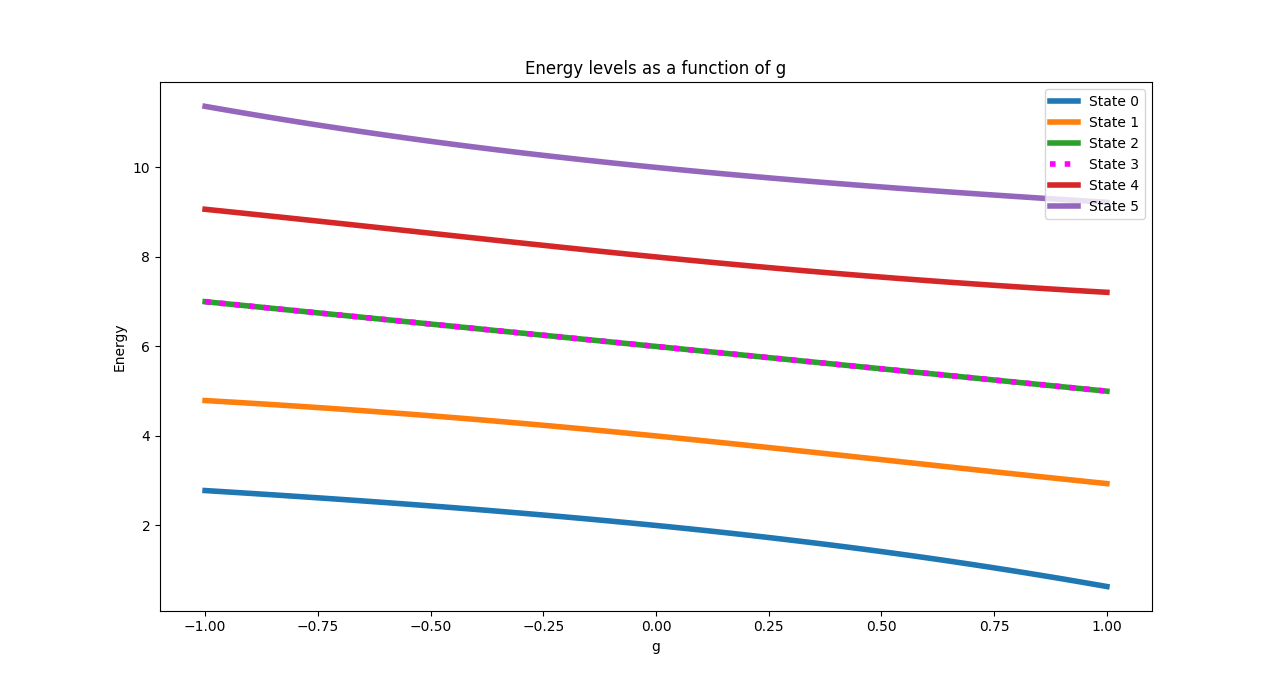
\includegraphics[scale = 0.5]{Figure_1.png}
    \caption{The Hamiltonian matrix for a system with no broken pairs and total spin of $S=0$, for the case of the four lowest single-particle states. Energies as a function of the strength of the interaction $g$.The dashed lines is to show the degeneracy of the states.}
    \label{fig:fig1}
\end{figure}
\begin{figure}[h]
    \centering
    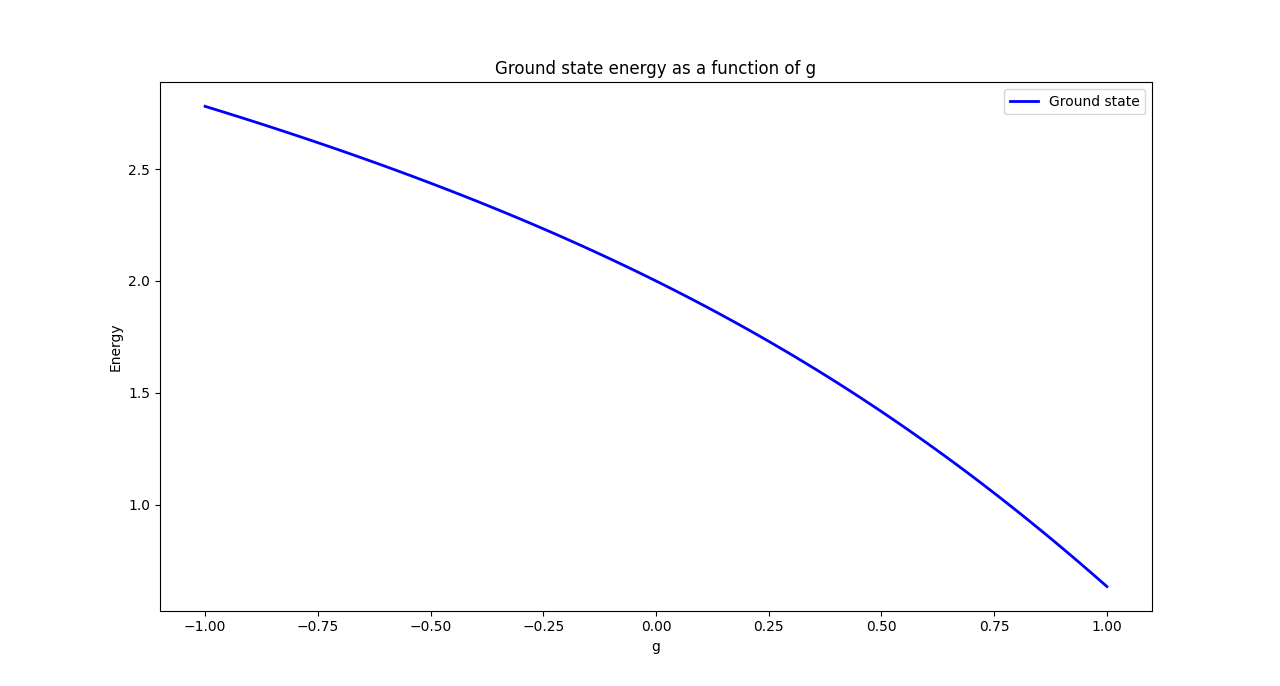
\includegraphics[scale = 0.5]{Figure_2.png}
    \caption{Ground state energy as a function of the interraction strength $g$.}
    \label{fig:fig2}
\end{figure}

\subsection*{c)}
In \ref{fig:fig1} the energy levels i show are from states $\ket{Φ_0}$ to $\ket{Φ_5}$, more explicitly:
$$
\ket{Φ_0} = P_1^+P_2^+ \ket{0}
\ket{Φ_1} = P_1^+P_3^+ \ket{0}
\ket{Φ_2} = P_1^+P_4^+ \ket{0}
$$
$$
\ket{Φ_3} = P_2^+P_3^+ \ket{0}
\ket{Φ_4} = P_2^+P_4^+ \ket{0}
\ket{Φ_5} = P_3^+P_4^+ \ket{0}
$$
For this part we want to make an approximation to the ground state energy. For this we will use at most two-particle two-holes excitations. Hence we will approximate the ground state energy by only using the states $\ket{Φ_0}$ and $\ket{Φ_4}$.\\
\begin{figure}[h!]
    \centering
    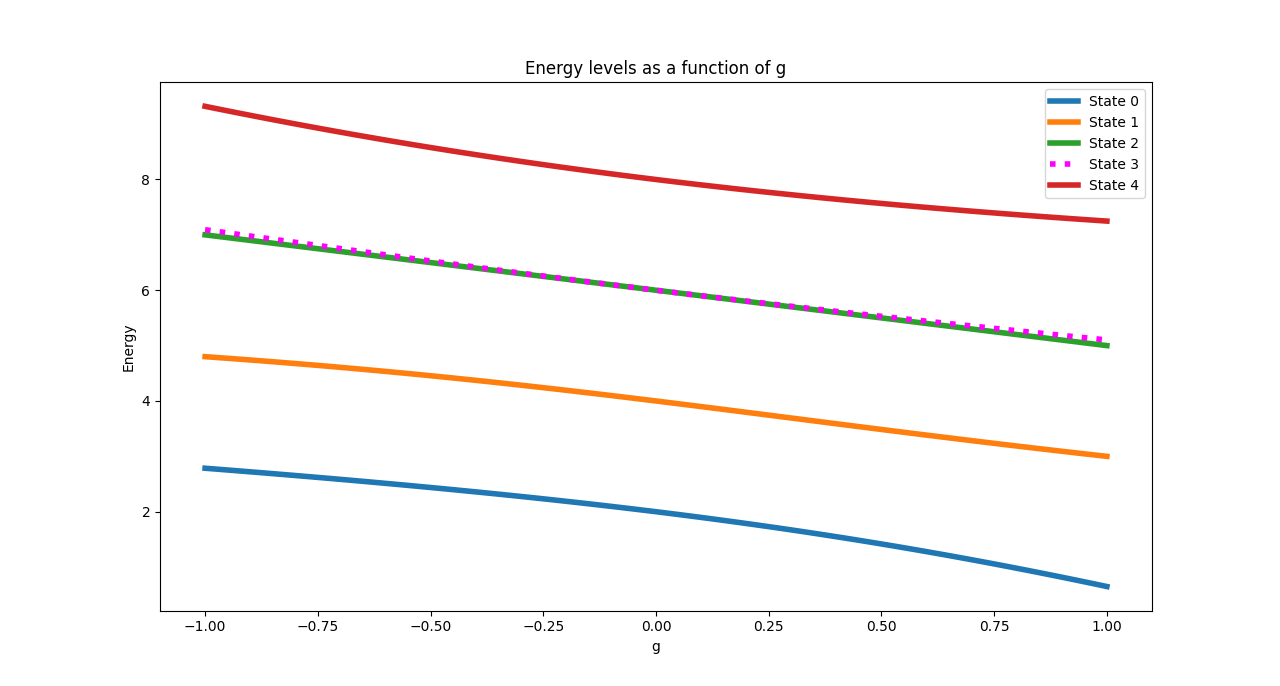
\includegraphics[scale = 0.5]{Figure_3.png}
    \caption{Excluding $ \ket{Φ_5}$. The Hamiltonian matrix for a system with no broken pairs and total spin of $S=0$, for the case of the four lowest single-particle states. Energies as a function of the strength of the interaction $g$}
    \label{fig:fig3}
\end{figure}
\begin{figure}[h!]
    \centering
    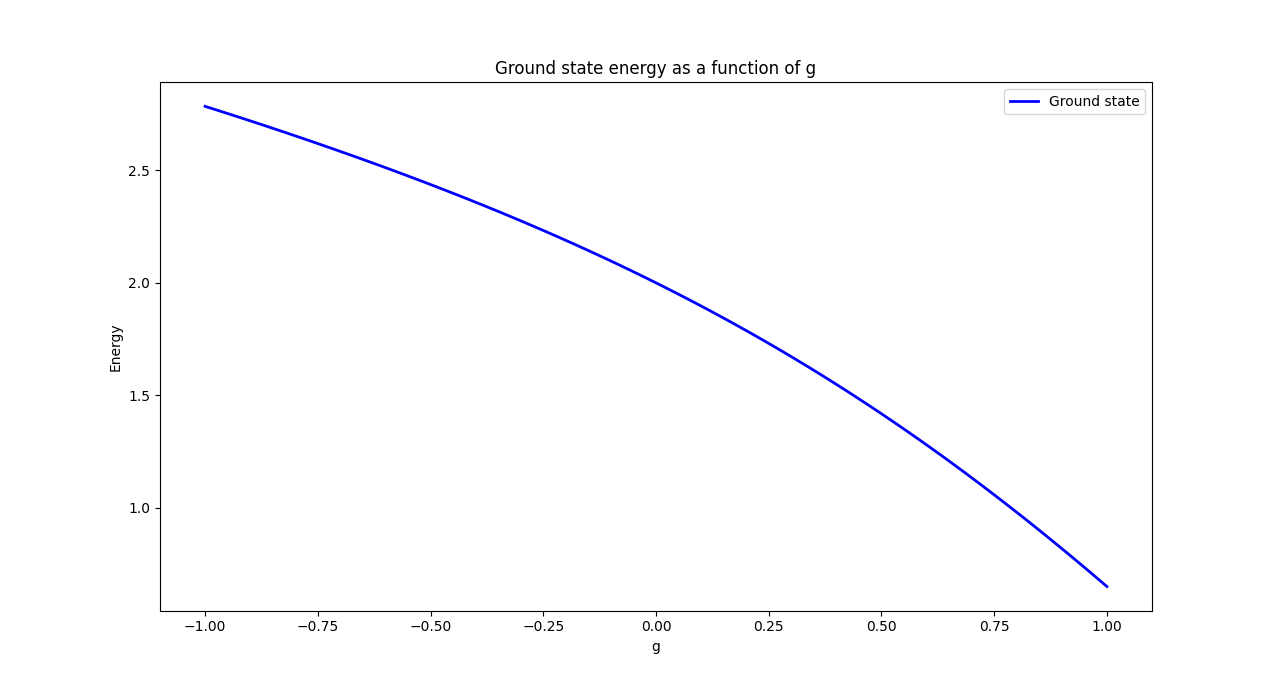
\includegraphics[scale = 0.5]{Figure_4.png}
    \caption{Ground state energy approximation as a function of the interraction strength $g$.}
    \label{fig:fig4}
\end{figure}
\begin{figure}[h!]
    \centering
    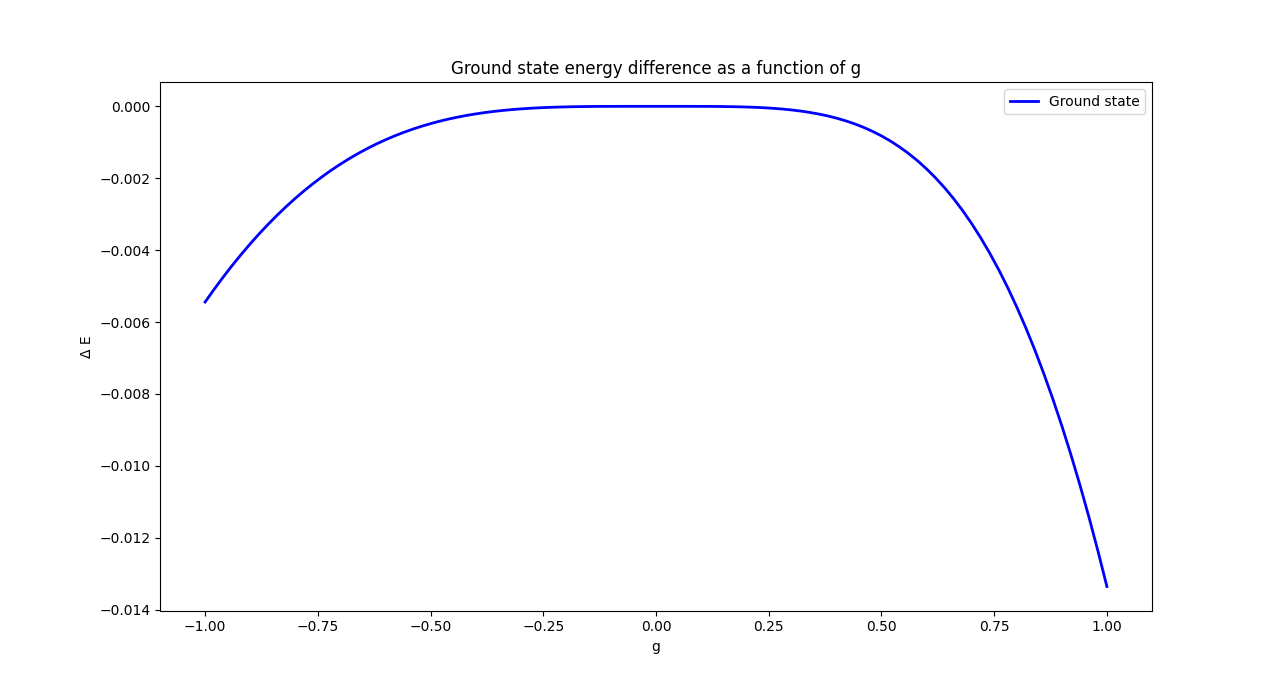
\includegraphics[scale = 0.5]{Figure_5.png}
    \caption{Difference between the ground state energy and the approximation as a function of the interraction strength $g$.}
    \label{fig:fig5}
\end{figure}
In \ref{fig:fig5} we show the energy difference between the approximation and the ground state energy. We can see that the approximation is very close to the ground state energy as the difference is very small. We can see that the energy difference is negative, meaning the approximated ground state has slightly higher energy than the true ground state energy.\\
TODO: add diagrammatic representation
\subsection*{d)}

The one-body operator $\hat{H}_0$ can be typically be expressed in terms of matrix elements $ \bra{ p} \hat{h}_0 \ket{q}$ as:
$$\hat{H}_0 = ∑_{pq}^{} \bra{p} \hat{h}_0 \ket{q}a_p ^{†} a_q$$
When normal ordering, we can adjust the term to:
$$a_p ^{†} a_q = \{a_p ^{†} a_q\} + δ_{pq ∈ i}$$
And from this we can write the one-body term as:
$$\hat{H}_0 = ∑_{pq}^{} \bra{p} \hat{h}_0 \ket{q}\{a_p ^{†} a_q\} + ∑_{pq}^{} \bra{p} \hat{h}_0 \ket{q} δ_{pq ∈ i}$$
Where the second term is a constant that represents the expectation value of the one-body operator in the refrence state:
$$∑_{pq}^{} \bra{p} \hat{h}_0 \ket{q} δ_{pq ∈ i} = \bra{Φ_0} \hat{H}_0 \ket{Φ_0} $$
From this we get 
$$\hat{H}_0 = ∑_{pq}^{} \bra{p} \hat{h}_0 \ket{q}\{a_p ^{†} a_q\} + \bra{Φ_0} \hat{H}_0 \ket{Φ_0}$$
Now applying the spesific case where $ \bra{ p} \hat{h}_0 \ket{ q} = (p-1) δ_{pq}$ and find that
$$\hat{H}_0 = ∑_{p σ}^{} (p-1) \{a_p ^{†} a_q\} + \bra{Φ_0} \hat{H}_0 \ket{Φ_0}$$
For the interraction term we will approach the normal ordering in a similar way. We can write the interraction term as:

$$ \hat{ H}_I = \frac{1}{4} ∑_{pqrs}^{} \bra{pq} \hat{ v} \ket{ rs}a_p ^{†} a_q ^{†} a_s a_r$$
where we can re-write the creation and annihilation operators as:
$$a_p ^{†} a_q ^{†} a_s a_r = \{a_p ^{†} a_q ^{†} a_s a_r\} + \wick{a_p ^{†} \c1a_q^{†} \c1a_s a_r} $$
$$ 
+ \wick{a_p ^{†} \c1a_q ^{†} a_s \c1a_r} + \wick{\c1a_p ^{†} a_q ^{†} \c1a_s a_r} + \wick{\c1a_p ^{†} a_q ^{†} a_s \c1a_r} + \wick{\c2a_p ^{†} \c1a_q ^{†} \c1a_s \c2a_r}
+ \wick{\c2a_p ^{†} \c1a_q ^{†} \c2a_s \c1 a_r}
$$

For this spesific case we will substitute $ \frac{1}{4} \bra{ pq} \hat{v}\ket{ rs}$ with $-\frac{g}{2}δ_{pq} δ_{rs} $. The interraction term can now be seperated into three parts:
\begin{itemize}
\item 1. The two body term, which arrises from the normal ordering of the creation and annihilation operators.
\item 2. The one body term, which comes from the single contractions. 
\item 3. The constant term, which comes from the double contractions.
\end{itemize}
From this we can construct a new normal ordered interraction term:
$$\hat{H}_I = -\frac{g}{2} ∑_{pq}^{} \{a_p ^{†} a_q ^{†} a_q a_p\} -\frac{g}{2} ∑_{pq}^{} a_{p σ}^{†}a_{p σ} + -\frac{g}{2} (δ_{pr}δ_{qs} + δ_{ps}δ_{qr}) $$ 

We can combine the one-body term into the first one we found, and we get:
$$
\hat{H}_0^N = ∑_{p σ}^{} (p-1)\{ a_{p σ}^{†} a_{p σ} \} -\frac{g}{2} ∑_{pq}^{} a_{p σ}^{†}a_{p σ}
$$
The normal ordered interraction term is:
$$  
\hat{V}^N = -\frac{g}{2} ∑_{pq}^{} \{a_p ^{†} a_q ^{†} a_q a_p\}
$$
and the refrence energy:
$$
E_0^{ref} = \bra{Φ_0} \hat{H}_0 \ket{Φ_0} -\frac{g}{2} ∑_{pq}^{} (δ_{pr}δ_{qs} + δ_{ps}δ_{qr}) = 2 - g
$$
where the values were obtained in the previous task.\\
The total normal ordered Hamiltonian is:
$$
\hat{H}^N = \hat{H}_0^N + \hat{V}^N + E_0^{ref}
$$
We now want to set up the standard Hartree Fock equations for the system, also known as the canonical Hartree-Fock equations. We begin by defining the single-particle operator $ \hat{ f}$, which for a general case is given by:
$$
\bra{ p} \hat{f} \ket{ q} = \bra{ p } \hat{H}_0 \ket{ q} + ∑_{j}^{} \bra{pj} \hat{ V} \ket{ qj}_{AS}
$$
where the subscript $AS$ indicates that the matrix elements are antisymmetrized. Due to the nature of the Hamiltionian, we have $ \bra{ p} \hat{ f} \ket{ q} = 0$ for $ p \neq q$. In second quantization we can write the single-particle operator as:
$$
\hat{ F}  = ∑_{ pq}^{ } \bra{ p} \hat{ f} \ket{ q}a_p ^{†} a_q = ∑_{p}^{} \bra{ p} \hat{ f} \ket{ p}a_p ^{†} a_p
$$
In writin the operator in normal order, we have:
$$
\wick{ \c1a_p ^{†} \c1a_p} = \{a_p ^{†} a_p\} + δ_{pp} 
$$
and thus:
$$
\hat{ F} = ∑_{p}^{} \bra{ p} \hat{ f} \ket{ p} \{a_p ^{†} a_p\} + ∑_{p}^{} \bra{ p} \hat{ f} \ket{ p} 
$$
The canonical Hartree-Fock equations are given by:
$$
\hat{ f} \ket{ p} = \epsilon_p \ket{ p}
$$
where $ \epsilon_p$ is the single-particle energy.


\subsection*{f)}


\subsection*{g)}


\end{document}